
%-------------------------------------------------------------------------------
%-------------------------------------------------------------------------------
%-------------------------------------------------------------------------------
\chapter{DS1 Centrale 2018}
%-------------------------------------------------------------------------------
%-------------------------------------------------------------------------------
%-------------------------------------------------------------------------------

À travers l'étude d'un jeu de société, ce sujet s'intéresse aux
mouvements de robots, qui possèdent des capacités
limitées de localisation. Avec le développement de la robotique,
plusieurs problèmes de ce type font l'objet de nombreuses
recherches :
parcours minimum pour examiner une surface donnée, stratégies
collectives avec plusieurs robots en interaction proche, nombre de
robots nécessaires pour que tous les points d'une surface avec obstacles
soient accessibles, etc.

Ce sujet porte sur la résolution de la situation pratique du jeu
{\sc Ricochet Robots} créé par Alex Randolph en 1999. Ce jeu se déroule
sur un plateau de $16 \times 16$ cases, avec $4$ robots (un robot principal et 3 autres indiscernables) et des murs. À
chaque mouvement, le joueur choisit un robot qu'il déplace, dans une des quatre
directions, jusqu'à ce qu'il rencontre un obstacle (un mur ou autre
robot). Le but est de trouver le nombre de coups minimal pour déplacer
le robot principal de son point de départ jusqu'à une case précise du
plateau. Un exemple en 8 coups est donné ci-dessous.
%-------------------------------------------------------------------------------
\begin{figure}[ht]
\begin{center}
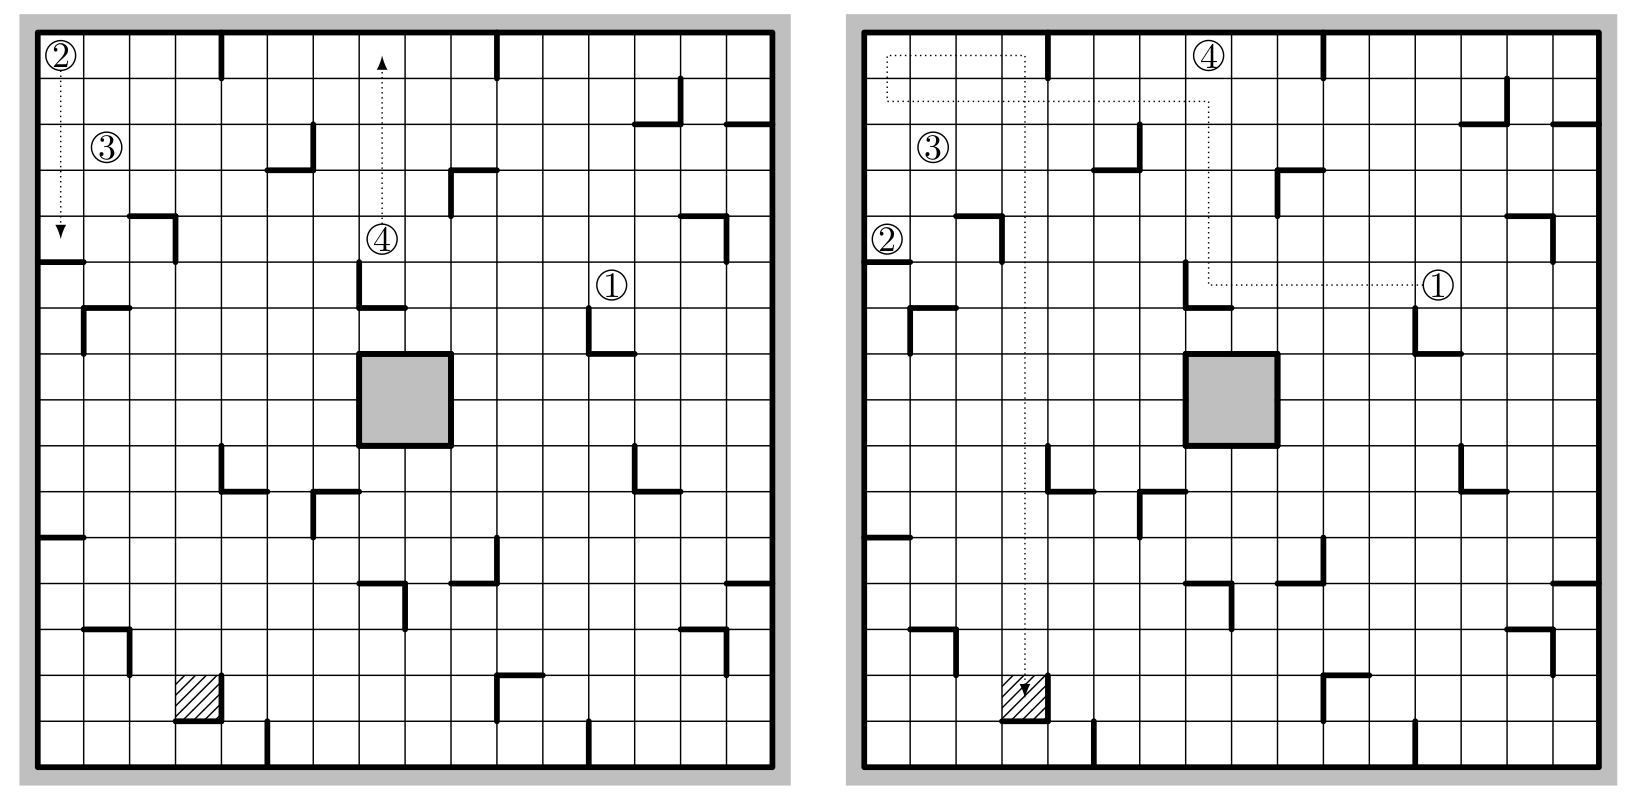
\includegraphics[width=\linewidth]{Figure1}
\caption{Le jeu des robots : le but est d'amener le robot 1 sur la case hachurée.\\
À gauche : deux déplacements des robots 2 et 4 ;
à droite : six déplacements du robot 1.\\
Le jeu est résolu en 8 mouvements (solution optimale)}
\end{center}
\end{figure}
%-------------------------------------------------------------------------------
\newpage

On rappelle la définition des fonctions suivantes, disponibles dans la
bibliothèque standard  :
\begin{itemize}
\item \type{Array.copy : 'a array -> 'a array} telle que l'appel
\type{Array.copy v} renvoie un nouveau tableau contenant les valeurs
contenues dans \type{v} ;

\item \type{Array.make : int -> 'a -> 'a array} telle que l'appel
\type{Array.make n x} renvoie un nouveau tableau de longueur \type{n}
initialisé avec des éléments égaux à \type{x} ;

\item \type{Array.make\_matrix : int -> int -> 'a -> 'a array array} telle que
l'appel 

\type{Array.make\_matrix p q x} renvoie une nouvelle matrice à
\type{p} lignes et \type{q} colonnes initialisée avec des éléments
égaux à \type{x}.
\end{itemize}
%-------------------------------------------------------------------------------
%-------------------------------------------------------------------------------
%-------------------------------------------------------------------------------
\section{Déplacement d’un robot dans une grille}
%-------------------------------------------------------------------------------
%-------------------------------------------------------------------------------
%-------------------------------------------------------------------------------
On considère pour le moment une grille sans robots du jeu Ricochet
Robots. Notons $N$ le nombre de cases par ligne et colonne de la grille
(16 dans le jeu originel). {\em Dans les fonctions demandées, on
supposera que $N$ est une variable globale}. On numérote chaque case par
un couple $(a,b)$ de $\{0, 1, \ldots, N-1\}^2$, correspondant à la ligne $a$ et à la
colonne $b$. On numérote également les lignes horizontales et verticales
séparant les cases à l’aide d’un entier de $\{0, 1, \ldots, N\}$, de sorte que la
case $(a,b)$ est délimitée par les lignes horizontales $a$ (au dessus)
et $a+1$ (en dessous), de même que par les lignes verticales $b$ (à
gauche) et $b+1$ (à droite).
%-------------------------------------------------------------------------------
\begin{figure}[ht]
\begin{center}
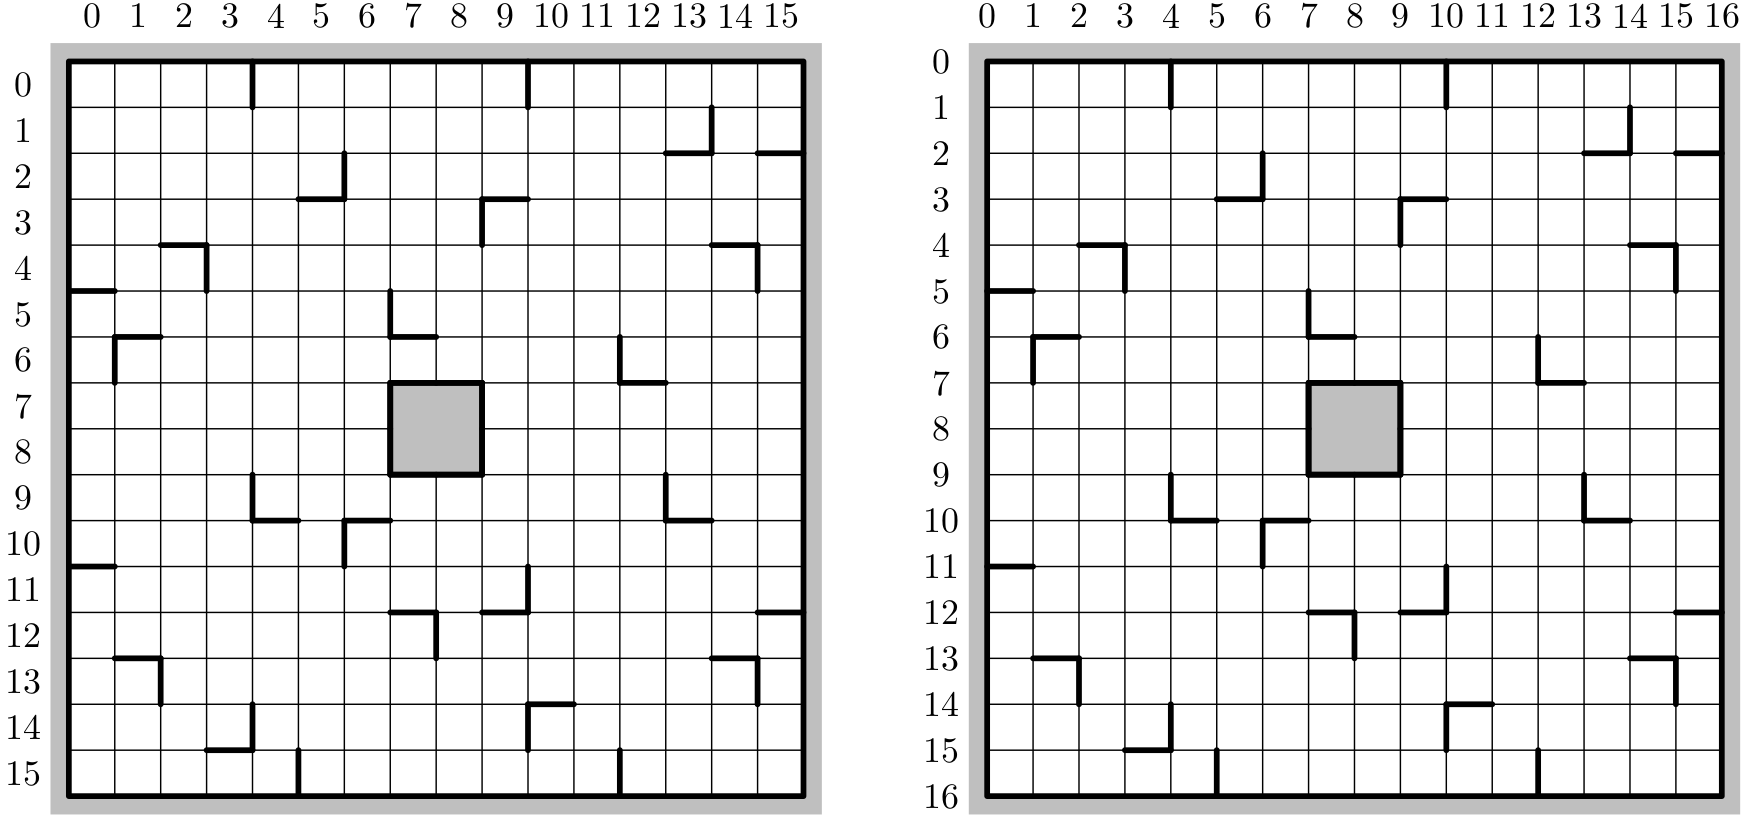
\includegraphics[width=\linewidth]{Figure2}
\caption{À gauche : numérotation des cases par ligne/colonne ;
à droite : numérotation des lignes horizontales et verticales
}
\end{center}
\end{figure}
%-------------------------------------------------------------------------------

\newpage

Pour représenter en OCaml la grille avec ses obstacles, on se donne
deux tableaux de taille $N$. Le premier contient les
obstacles verticaux sur chacune des lignes, le second contient les
obstacles horizontaux sur chacune des colonnes. Un obstacle est donné
par le numéro de la ligne (verticale ou horizontale) auquel il
appartient. Les obstacles sur une ligne (ou colonne) sont donnés sous la
forme d’un tableau ordonné dans l’ordre croissant.
Par exemple, la représentation du plateau ci-dessus serait
%-------------------------------------------------------------------------------
\begin{lstlisting}
let obstacles_lignes = 
  [| [|0; 4; 10; 16|]; [|0; 14; 16|]; [|0; 6; 16|];
     [|0; 9; 16|]; [|0; 3; 15; 16|]; [|0; 7; 16|]; 
     [|0; 1; 12; 16|]; [|0; 7; 9; 16|]; [|0; 7; 9; 16|]; 
     [|0; 4; 13; 16|]; [|0; 6; 16|]; [|0; 10; 16|]; 
     [|0; 8; 16|]; [|0; 2; 15; 16|]; [|0; 4; 10; 16|]; 
     [|0; 5; 12; 16|] |];;

let obstacles_colonnes = 
  [| [|0; 5; 11; 16|]; [|0; 6; 13; 16|]; [|0; 4; 16|];
     [|0; 15; 16|]; [|0; 10; 16|]; [|0; 3; 16|]; 
     [|0; 10; 16|]; [|0; 6; 7; 9; 12; 16|]; 
     [|0; 7; 9; 16|]; [|0; 3; 12; 16|]; [|0; 14; 16|]; 
     [|0; 16|]; [|0; 7; 16|]; [|0; 2; 10; 16|]; 
     [|0; 4; 13; 16|]; [|0; 2; 12; 16|] |];;
\end{lstlisting}
%-------------------------------------------------------------------------------

Notez que les bordures de la grille sont considérées comme des
obstacles. Ainsi, les entiers $0$ et $N$ sont présents dans les tableaux
associés à chaque ligne/colonne.

%-------------------------------------------------------------------------------
%-------------------------------------------------------------------------------
\begin{Exercise}\it
Écrire une fonction \type{dichotomie a t} de signature \type{int -> int array -> int} telle que si \type{t} est un tableau d’entiers strictement
croissants et \type{a} un élément supérieur ou égal au premier élément du
tableau et strictement inférieur au dernier, la fonction renvoie
l’unique indice \type{i} tel que $\type{t.(i)} \leq \type{a} < \type{t.(i+1)}$.
La fonction doit avoir une complexité logarithmique en la
taille du tableau.
\end{Exercise}
%-------------------------------------------------------------------------------
\begin{Answer}
La fonction demandée s'appelle \type{dichotomie} et on demande une complexité logarithmique : on va utiliser une recherche par dichotomie. L'idée est de travailler avec deux indices, $i$ et $j$ tels que \type{t.(i) <= a < t.(j)} : c'est un invariant de boucle.
\begin{lstlisting}
let dichotomie a t =
  let n = Array.length t in
  let i = ref 0 in
  let j = ref (n -1) in
    while !i + 1 < !j do
      let c = (!i + !j)/2 in
      if a < t.(c) then j := c
                   else i := c done;
    !i;;
\end{lstlisting}

On peut aussi donner une écriture récursive
\begin{lstlisting}
let dichotomie a t =
  let rec aux i j =
    if j = i + 1
    then i
    else let c = (i+j)/2 in
         if a < t.(c)
         then aux i c
         else aux c j
  in aux 0 (Array.length t  - 1);;
\end{lstlisting}

On suppose qu'on a $j-i \le 2^p$ on a alors $i+2^{p-1} \le c \le j-2^{p-1}$, les nouvelles valeurs de $i$ et $j$, $i'$ et $j'$, vérifient alors $j'-i' \le 2^{p-1}$. Si on a $2^{N-1} < n-1-0\le 2^N$ alors, après au plus $N$ passages dans la boucle on a $j-i\le 1$ et la boucle termine.

La complexité est donc majorée par $N$ qui est un ${\cal O}\bigl(\log(n)\bigr)$.
\end{Answer}
%-------------------------------------------------------------------------------
%-------------------------------------------------------------------------------

\medskip


On considère un robot positionné en $(a, b)$, avec $0 \leq a,b < N$. Il
peut se déplacer dans les quatre directions cardinales
ouest/est/nord/sud représentées ci-dessous

\begin{center}
\begin{tikzpicture}
\node (O) at (0,0) [circle, draw, minimum width=2ex] {};
\draw[->, densely dotted] (O) -- (0,1) node[above] {nord} ;
\draw[->, densely dotted] (O) -- (1,0) node[right] {est} ;
\draw[->, densely dotted] (O) -- (-1,0) node[left] {ouest} ;
\draw[->, densely dotted] (O) -- (0,-1) node[below] {sud} ;
\end{tikzpicture}
\end{center}
%-------------------------------------------------------------------------------
%-------------------------------------------------------------------------------
\begin{Exercise}\it
Écrire une fonction
\type{deplacements\_grille (a,b)} de signature \type{int * int -> (int * int) array} fournissant les 4 cases atteintes par les déplacements en
question, sous forme d’un tableau à 4 éléments (ouest/est/nord/sud). Si le robot ne peux pas bouger
dans une direction donnée (car il est contre un obstacle), on considérera
que le résultat du déplacement dans cette direction est la case $(a,b)$ elle-même. 

Les deux tableaux \type{obstacles\_lignes} et \type{obstacles\_colonnes} sont des
variables globales.
\end{Exercise}
%-------------------------------------------------------------------------------
\begin{Answer}
On considère la case $(a,b)$.

Sur la ligne d'ordonnée $b$ les obstacles sont aux positions dans \type{obstacles\_ligne.(b)}, noté \type{t}.

Si $p$ est la longueur de \type{t} on a \type{t.(0) = 0 <= a < n = t.(p-1)} ; on peut calculer \type{dichotomie a t}. On trouve un indice $i$ tel que \type{t.(i) <= a < t.(i+1)}. Ainsi \type{t.(i)} est le dernier obstacle à gauche de $a$ et \type{t.(i+1)} est le premier obstacle à droite de $a$ (sur la ligne $b$).

On en déduit que le déplacement à gauche va s'arrêter à la case \type{t.(i)} et le déplacement à droite va s'arrêter à la case \type{t.(i+1) - 1}.
De même pour les déplacement nord-sud.
\begin{lstlisting}
let deplacement_lignes (a, b) =
  let t = obstacles_lignes.(b) in
  let i = dichotomie a t in
  let ouest = t.(i) in
  let est = t.(i+1) -1 in
  let s = obstacles_colones.(a) in
  let j = dichotomie b t in
  let nord = s.(j) in
  let sud = s.(j+1) -1 in
  [| (ouest, b); (est, b); (a, nord); (a, sud) |];;
\end{lstlisting}

Comme on a utilisé deux fois \type{dichotomie} donc la complexité est en ${\cal O}\bigl(\log(n)\bigr)$.

\newpage
\end{Answer}
%-------------------------------------------------------------------------------
%-------------------------------------------------------------------------------
\begin{Exercise}\it
Écrire une fonction
\type{matrice\_deplacements ()}, de type \type{unit ->
(int * int) array array array} produisant une matrice \type{m} telle que
\type{m.(a).(b)} contienne le arrayeur des déplacements possibles pour un
robot depuis la case $(a, b)$, et ce pour tous $0 \leq a,b < N$. Donner
la complexité de création de la matrice.
\end{Exercise}
%-------------------------------------------------------------------------------
\begin{Answer}
On construit une matrice vide qu'on remplit case par case avec la fonction précédente
\begin{lstlisting}
let matrice_deplacements () =
  let m = Array.make_matrix n n [||] in
  for a = 0 to n - 1 do 
    for b = 0 to n - 1 do
      m.(a).(b) <- deplacements_grille (a, b) done done;
  m;;
\end{lstlisting}
En raison des deux boucles imbriquées, la complexité est en ${\cal O}\bigl(n^2log(n)\bigr)$.
\end{Answer}
%-------------------------------------------------------------------------------
%-------------------------------------------------------------------------------

\medskip

On cherche maintenant à intégrer les positions d’autres robots
dans le déplacement d’un robot. On utilise la fonction précédente pour
créer une matrice \type{mat\_deplacements} que l’on considérera comme
globale.

%-------------------------------------------------------------------------------
%-------------------------------------------------------------------------------
\begin{Exercise}\it
Écrire une fonction \type{modif t (a,b) (c,d)} de signature

\type{(int * int) array -> int * int -> int * int -> unit}

telle que si
\type{t} est le tableau de taille 4 donnant les déplacements
ouest/est/nord/sud d’un robot placé en $(a,b)$ dans la grille ne
contenant pas d’autres robots, et $(c,d)$ la position d’un autre robot,
alors la fonction modifie si nécessaire le tableau \type{t} en prenant en
compte le robot en $(c,d)$.
\end{Exercise}
%-------------------------------------------------------------------------------
\begin{Answer}
Un robot en $(c, d)$ devient un obstacle possible en $c$ pour les déplacements vers l'ouest des points $(a, d)$ avec $a > c$ et un obstacle possible en $c$ pour les déplacements vers l'est des points $(a, d)$ avec $a < c$.
On suppose ici que les deux points sont distincts.

On a choisi de faire 4 tests séparés pour que la structure reste lisible.
\begin{lstlisting}
let modif t (a, b) (c, d) =
  if b = d && a > c
  then t.(0) <- (max (c+1) (snd t.(0)), b);
  if b = d && a < c
  then t.(1) <- (min (c-1) (snd t.(1)), b);
  if a = c && b > d
  then t.(2) <- (a, max (d+1) (snd t.(2)));
  if a = c && b < d
  then t.(3) <- (a, min (d-1) (snd t.(3)));;
\end{lstlisting}
\end{Answer}
%-------------------------------------------------------------------------------
%-------------------------------------------------------------------------------

\medskip

On s’intéresse maintenant au déplacement d’un robot situé en
$(a,b)$ dans la grille, avec d’autres robots éventuellement présents,
dont les positions sont stockées dans une liste.
%-------------------------------------------------------------------------------
%-------------------------------------------------------------------------------
\begin{Exercise}\it
Déduire des questions précédentes une fonction
\type{deplacements\_robots (a,b) q} de signature

\type{int * int -> (int * int) list -> (int * int) array}

donnant les
déplacements ouest/est/nord/sud d’un robot situé en $(a,b)$ dans la
grille, les positions des autres robots étant stockées dans la liste
\type{q}. On ne modifiera pas la matrice \type{mat\_deplacements} : on
souhaite une copie modifiée de \type{mat\_deplacements.(a).(b)}.
\end{Exercise}
%-------------------------------------------------------------------------------
\begin{Answer}
On commence par copier le vecteur de déplacements de la matrice de déplacements. On traite la liste à l'aide d'une fonction récursive auxiliaire.
\begin{lstlisting}
let deplacements_robots (a, b) q =
  let t = Array.copy mat_deplacements.(a).(b) in
  let rec aux q = 
    match q with
    |[] -> ()
    |(c, d)::reste -> modif t (a, b) (c, d); aux reste 
  in maj q;   t;;
\end{lstlisting}
\end{Answer}
%-------------------------------------------------------------------------------
%-------------------------------------------------------------------------------
\begin{Exercise}\it
Si on suppose que la solution optimale demande au plus $k$ mouvements,
une solution possible pour résoudre le jeu Ricochet Robots consiste à
générer toutes les suites possibles de $k$ déplacements.
Avec 4 robots en tout, estimer la complexité d’une telle approche (on
utilisera la notation ${\cal O}$).
\end{Exercise}
%-------------------------------------------------------------------------------
\begin{Answer}
À chaque itération, on peut déplacer chacun des 4 robots dans une des 4 directions : cela fait un total de 16 déplacements possibles. 

On en déduit que le nombre de suites de $k$ déplacements est $16^k$.

La complexité est donc un ${\cal O}(16^k)$ : elle n'est possible que pour des valeurs très petites de $k$.
\end{Answer}
%-------------------------------------------------------------------------------
%-------------------------------------------------------------------------------

\medskip

La suite du problème a pour objet de proposer une solution
plus efficace pour la résolution du jeu Ricochet Robots.
%-------------------------------------------------------------------------------
%-------------------------------------------------------------------------------
%-------------------------------------------------------------------------------
\section{Quelques fonctions utilitaires}
%-------------------------------------------------------------------------------
%-------------------------------------------------------------------------------
%-------------------------------------------------------------------------------
\subsection{Une fonction de tri}
%-------------------------------------------------------------------------------
%-------------------------------------------------------------------------------
\begin{Exercise}\it
Écrire une fonction \type{insertion x q} de signature \type{'a -> 'a list
-> 'a list} prenant en entrée un élément \type{x} et une liste \type{q}
triée dans l’ordre croissant, et renvoyant une liste triée dans l’ordre
croissant, constituée des éléments de \type{q} et \type{x}.
\end{Exercise}
%-------------------------------------------------------------------------------
\begin{Answer}
\begin{lstlisting}
let rec insertion x liste = 
  match liste with
  |[] -> [x]
  |y::reste when x <= y -> x::liste
  |y::reste -> y::(insertion x reste);;
\end{lstlisting}
\newpage
\end{Answer}
%-------------------------------------------------------------------------------
%-------------------------------------------------------------------------------
\begin{Exercise}\it
En déduire une fonction \type{tri\_insertion q} de signature \type{'a list
-> 'a list} permettant de trier une liste dans l’ordre croissant.
\end{Exercise}
%-------------------------------------------------------------------------------
\begin{Answer}
\begin{lstlisting}
let rec tri_insertion liste = 
  match liste with
  |[] -> []
  |t::reste -> insertion t (tri_insertion reste);;
\end{lstlisting}
\end{Answer}
%-------------------------------------------------------------------------------
%-------------------------------------------------------------------------------
\begin{Exercise}\it
Rappeler la complexité de ce tri dans le pire et le meilleur cas. Que
peut-on dire de la complexité si dans la liste \type{q}, tous les
éléments excepté peut-être un sont dans l’ordre croissant ?
\end{Exercise}
%-------------------------------------------------------------------------------
\begin{Answer}
Dans le pire des cas, la complexité est quadratique (par exemple pour une liste décroissante). 

Dans le meilleur des cas, la complexité est linéaire (pour une liste triée). 

Soit $L = (a_0, \dots, a_k, x, a_{k+1}, \dots a_{n-1})$ une liste, telle que seul l'élément $x$ n'est pas à sa place. 

le tri se fait en commençant par la fin.

\begin{itemize} 
    \item Le tri de la sous-liste triée $(a_{k+1}, \dots,  a_{n-1})$ est en $O(1)$ pour chaque élément.
    \item Si $x > a_{k+1}$, alors l'insertion de $x$ se fera en l'insérant progressivement à droite jusqu'à sa position. Cette insertion est alors en $O(n)$, et les insertions suivantes se feront alors en $O(1)$ car la liste est triée. Au final, la complexité est en $O(n)$. 
    \item Si $x < a_k$, alors l'insertion de $x$ se fera en $O(1)$. Les éléments qui précèdent sont, pour certains, plus grands que $x$ : ils seront insérés derrière $x$, ce qui se fera avec deux appels à la fonction \texttt{insertion}, donc en $O(1)$. Les autres se feront en un seul appel. 
    
    Au final, la complexité est en $O(N)$.
\end{itemize} 

Quand un seul élément n'est pas à sa place, la complexité est en $O(N)$.
\end{Answer}
%-------------------------------------------------------------------------------
%-------------------------------------------------------------------------------
\subsection{Quelques fonctions sur les listes}
%-------------------------------------------------------------------------------
%-------------------------------------------------------------------------------
\begin{Exercise}\it
Écrire une fonction \type{mem1 x q} de signature \type{'a -> ('a * 'b)
list -> bool} testant l’appartenance d’un couple dont le premier élément
est \type{x} dans la liste \type{q}.
\end{Exercise}
%-------------------------------------------------------------------------------
\begin{Answer}
\begin{lstlisting}
let rec mem1 x liste = 
  match liste with
  |[] -> false
  |(a, b)::reste when x = a -> true
  |t::reste-> mem1 x reste;;
\end{lstlisting}
\end{Answer}
%-------------------------------------------------------------------------------
%-------------------------------------------------------------------------------

\begin{Exercise}\it
Écrire une fonction \type{assoc x q} de signature \type{'a -> ('a * 'b)
list -> 'b} renvoyant, s’il existe, l’élément \type{y} du premier couple
\type{(x,y)} appartenant à la liste \type{q}.
\end{Exercise}
%-------------------------------------------------------------------------------
\begin{Answer}
\begin{lstlisting}
let assoc x liste = 
  match liste with
  |[] -> failwith "Element non present"
  |(a, b)::reste when x = a -> b
  |t::reste-> assoc x reste;;
\end{lstlisting}
\end{Answer}
% %-------------------------------------------------------------------------------
% %-------------------------------------------------------------------------------
% \subsection{Implantation d’une structure de file}
% %-------------------------------------------------------------------------------
% %-------------------------------------------------------------------------------
% On rappelle que l’on peut facilement implanter une structure de file à
% l’aide de deux listes : une des listes est utilisée pour rajouter des
% éléments, l’autre pour enlever des éléments. On définit ainsi le type
% %-------------------------------------------------------------------------------
% \begin{lstlisting}
% type 'a file = {mutable entree: 'a list; mutable sortie: 'a list};;  
% \end{lstlisting}
% %-------------------------------------------------------------------------------
% Lorsqu’on veut retirer un élément de la file alors que la deuxième liste
% est vide, on remplace celle-ci par la première, renversée.

% \newpage

% On pourra utiliser les fonctions suivantes, qui permettent de
% manipuler une file ainsi définie :
% %-------------------------------------------------------------------------------
% \begin{itemize}
% \item \type{creer\_file\_vide : unit -> 'a file} crée une file vide,
% \item \type{est\_vide\_file : 'a file -> bool}  teste si une file est vide,
% \item \type{enfiler : 'a file -> 'a -> unit}  ajoute un élément à une file,
% \item \type{defiler : 'a file -> 'a}  supprime l’élément en tête de file et le renvoie.
% \end{itemize}
% %-------------------------------------------------------------------------------
% On pourra supposer dans la suite que ces fonctions sont écrites de
% sorte que toute suite de $p$ opérations \type{enfiler}/\type{defiler} à partir d’une
% file vide (ne produisant pas d’erreur) se fait en complexité ${\cal O}(p)$.
%-------------------------------------------------------------------------------
%-------------------------------------------------------------------------------
%-------------------------------------------------------------------------------
\section{Tables de hachage}
%-------------------------------------------------------------------------------
%-------------------------------------------------------------------------------
%-------------------------------------------------------------------------------
Dans l’optique de résoudre le problème du jeu des robots, nous allons
travailler sur un graphe dont les sommets seront étiquetés par les
positions des robots. Le nombre de sommets possibles étant élevé, il est
nécessaire d’utiliser une structure de données adaptée pour
travailler sur ce graphe. Nous allons donc réaliser une structure
de dictionnaire permettant, en particulier, de tester facilement si un
sommet a déjà été vu ou non et d’associer un sommet à chaque sommet
découvert.

Une structure de dictionnaire est un ensemble de couples
$(\text{clé},\text{élément})$, les clés (nécessairement distinctes)
appartenant à un même ensemble $K$, les éléments à un ensemble $E$. La
structure doit garantir les opérations suivantes :
%-------------------------------------------------------------------------------
\begin{itemize}
\item recherche d’un élément connaissant sa clé ;
\item ajout d’un couple $(\text{clé},\text{élément})$ ;
\item suppression d’un couple connaissant sa clé.
\end{itemize}
%-------------------------------------------------------------------------------
Une structure de dictionnaire peut-être réalisée à l’aide d’une table
de hachage. Cette table est implantée dans un tableau de $w$ listes
(appelées {\em alvéoles}) de couples $(\text{clé},\text{élément})$. Ce
tableau est organisé de façon à ce que la liste d’indice $i$ contienne
tous les couples $(k,e)$ tels que $h_w(k)=i$ où $h_w : K \mapsto \{0, 1, \ldots, w-1\}$ s’appelle {\em fonction de hachage}. 
On appelle $w$ la {\em largeur de la table} de hachage et $h_w(k)$ le {\em haché} de la clé $k$.

Ainsi pour rechercher ou supprimer l’élément de clé $k$, on commence
par calculer son haché qui détermine l’alvéole adéquate et on est
alors ramené à une action sur la liste correspondante. De même pour
ajouter un nouvel élément au dictionnaire on l’ajoute à l’alvéole
indiquée par le haché de sa clé.
%-------------------------------------------------------------------------------
%-------------------------------------------------------------------------------
\subsection{Une famille de fonctions $h_w$}
%-------------------------------------------------------------------------------
%-------------------------------------------------------------------------------
Nous commençons par nous doter d’une famille de fonctions $h_w$, pour les listes
de couples de $\{0, 1, \ldots, N-1\}^2$. Un hachage naturel d’une liste comportant
les couples $(a_i, b_i)_{0 \leq i < p}$ avec $0 \leq a_i, b_i < N-1$ est
donnée par :
\[
P_w(N)=\left(\sum_{i=0}^{p-1}(a_i+b_iN)N^{2i}\right) \text{ modulo } w
\]
Autrement dit, on évalue le polynôme dont les coefficients sont donnés
par les $a_i$ et $b_i$ en $N$, et on ne considère que le reste dans la
division euclidienne par $w$. On rappelle qu’on a supposé que $N$ est
une variable globale.
%-------------------------------------------------------------------------------
%-------------------------------------------------------------------------------
\begin{Exercise}\it
Écrire une fonction récursive \type{hachage\_liste w q} de signature
\type{int -> (int * int) list -> int} calculant la quantité précédente.
\end{Exercise}
%-------------------------------------------------------------------------------
\begin{Answer}
Il n'y a pas de fonction puissance en Caml. On va utiliser la règle de Hörner pour faire le calcul : elle évite de calculer les puissances de $N$.
\begin{lstlisting}
let rec hachage_liste w liste = 
  match liste with
  |[] -> 0
  |(a, b)::reste -> 
    ((hachage_liste w reste)*n*n + a + b*n) mod w;;  
\end{lstlisting}
\end{Answer}
%-------------------------------------------------------------------------------
\newpage
%-------------------------------------------------------------------------------
\subsection{Tables de hachage de largeur fixée}
%-------------------------------------------------------------------------------
%-------------------------------------------------------------------------------
% Dans cette sous-section, on fixe une largeur de hachage $w$. Un bon
choix pour $w$ serait par exemple un nombre premier ni trop petit, ni
trop grand, comme 997. Pour les listes, on considérerait alors la
fonction de hachage $h_{997}$ donnée en OCaml par
\type{hachage\_liste 997}. On définit en toute généralité le type suivant:

\begin{lstlisting}
type ('a, 'b) table_hachage = {
  hache: 'a -> int;
  donnees: ('a * 'b) list array;
  largeur: int};;
\end{lstlisting}
%-------------------------------------------------------------------------------
%-------------------------------------------------------------------------------
\subsubsection{Implantation de la structure de dictionnaire}
%-------------------------------------------------------------------------------
%-------------------------------------------------------------------------------
\begin{Exercise}\it
Écrire une fonction \type{creer\_table h w} de signature \type{('a -> int)
-> int -> ('a, 'b) table\_hachage} telle que \type{creer\_table h w}
renvoie une nouvelle table de hachage vide de largeur \type{w} munie de
la fonction de hachage \type{h}.
\end{Exercise}
%-------------------------------------------------------------------------------
\begin{Answer}
 On n'a pas besoin des type \type{'a} et \type{'b} : on remplit le tableaux de listes vides.
\begin{lstlisting}
let creer_table h w =
  let tab = Array.make w [] in
  {hache = h; donnees = tab; largeur = w};; 
\end{lstlisting}
On notera que \type{largeur} est inutile, c'est la longueur de \type{donnees}.
\end{Answer}
%-------------------------------------------------------------------------------
%-------------------------------------------------------------------------------

\begin{Exercise}\it
Écrire une fonction \type{recherche t k} de signature \type{('a, 'b)
table\_hachage -> 'a -> bool} renvoyant un booléen indiquant si la clé
$k$ est présente dans la table $t$. On pourra utiliser les fonctions de
la partie {\bf 2}.
\end{Exercise}
%-------------------------------------------------------------------------------
\begin{Answer}
 On utilise les fonctions de la partie précédente pour chercher dans la liste définie par la fonction de hachage.
\begin{lstlisting}
let recherche table k =
  let ind = table.hache k in
  let liste = table.donnees.(ind) in
  mem1 k liste;;
\end{lstlisting}
\end{Answer}
%-------------------------------------------------------------------------------
%-------------------------------------------------------------------------------

\begin{Exercise}\it
Écrire une fonction \type{element t k} de signature \type{('a, 'b)
table\_hachage -> 'a -> 'b} renvoyant l’élément $e$ associé à la clé
$k$ dans la table $t$, si cette clé est bien présente dans la table.
\end{Exercise}
%-------------------------------------------------------------------------------
\begin{Answer}
\begin{lstlisting}
let element table k =
  let ind = table.hache k in
  let liste = table.donnees.(ind) in
  assoc k liste;;
\end{lstlisting}
\end{Answer}
%-------------------------------------------------------------------------------
%-------------------------------------------------------------------------------

\begin{Exercise}\it
Écrire une fonction \type{ajout t k e} de signature \type{('a, 'b)
table\_hachage -> 'a -> 'b -> unit} ajoutant l’entrée $(k, e)$ à la
table de hachage $t$. On n’effectuera aucun changement si la clé est
déjà présente.
\end{Exercise}
%-------------------------------------------------------------------------------
\begin{Answer}
\begin{lstlisting}
 let ajout table k e =
  if not (recherche table k) 
  then let ind = table.hache k in
      table.donnees.(ind) <- (k, e) :: table.donnees.(ind);;
\end{lstlisting}
\end{Answer}
%-------------------------------------------------------------------------------
%-------------------------------------------------------------------------------

\begin{Exercise}\it
Écrire enfin une fonction \type{suppression t k} de signature \type{('a,
'b) table\_hachage -> 'a -> unit} supprimant l’entrée de la clé $k$
dans la table $t$. On n’effectuera aucun changement si la clé n’est pas
présente.
\end{Exercise}
%-------------------------------------------------------------------------------
\begin{Answer}
On écrit une fonction auxiliaire qui supprime un élément d'une liste.
\begin{lstlisting}
let suppression table k =
  let rec supp liste = 
    match liste with
    |[] -> []
    |(a, b)::reste when a = k -> reste
    |x::reste -> x::(supp reste) in
  let ind = ind = table.hache k in
  table.donnees.(ind) <- supp t.donnees.(ind);;
\end{lstlisting}
\end{Answer}
%-------------------------------------------------------------------------------
%-------------------------------------------------------------------------------
\subsubsection{Étude de la complexité de la recherche d’un élément}
%-------------------------------------------------------------------------------
%-------------------------------------------------------------------------------
Nous étudions ici la complexité de la recherche d’une clé dans une table de
hachage. Dans le pire cas, toutes les clés sont hachées vers la même
alvéole, ainsi la complexité de la recherche d’une clé dans une table de
hachage n’est pas meilleure que la recherche dans une liste. Cependant,
si la fonction de hachage $h_w$ est bien choisie, on peut espérer
que les clés vont se répartir de façon apparemment aléatoire dans les
alvéoles, ce qui donnera une complexité bien meilleure.

Nous faisons donc ici l’hypothèse de {\em hachage uniforme simple} : pour
une clé donnée, la probabilité d’être hachée dans l’alvéole $i$ est
$1/w$, indépendante des autres clés. On note $n$ le
nombre de clés stockées dans la table et on appelle $\alpha=n/w$ le
{\em facteur de remplissage} de la table. On
suppose de plus, que le calcul du haché d’une clé se fait
en temps constant.
%-------------------------------------------------------------------------------
%-------------------------------------------------------------------------------
\begin{Exercise}\it
On se donne une clé $k$ non présente dans la table. Montrer que
l’espérance de la complexité de la recherche de $k$ dans la table est un
${\cal O}(1+\alpha)$.
\end{Exercise}
%-------------------------------------------------------------------------------
\begin{Answer}La complexité est donc la somme de la complexité du calcul du hache et de la recherche dans l'alvéole. Pour une clé qui n'est pas trouvée, la complexité de la recherche est proportionnelle à la longueur de la liste.

On note $L_i$, la longueur de la liste dans l'alvéole d'indice $i$.

La complexité moyenne d'une recherche quand le hache est $i$ est donc majorée par $K(1+L_i)$, où $K$ majore la complexité du calcul de l'indice  et celle d'une comparaison.
La complexité moyenne vérifie donc 
\[C(n) \le \sum_{i=0}^{w-1}\frac 1w K(1+L_i)
=\frac Kw\left(\sum_{i=0}^{w-1}1+\sum_{i=0}^{w-1}L_i\right)
=\frac Kw\left(w+n\right) = K(1+\alpha)\]
\end{Answer}
%-------------------------------------------------------------------------------
%-------------------------------------------------------------------------------
\begin{Exercise}\it
On prend au hasard une clé présente dans la table ; toutes les clés sont
équiprobables. Montrer qu’alors la recherche de la clé se fait en
${\cal O}(1+\alpha)$, en moyenne sur toutes les clés présentes.
\end{Exercise}
%-------------------------------------------------------------------------------
\begin{Answer} L'équi-probabilité porte ici sur les $n$ valeurs dans la table, pas sur les $w$ alvéoles.

On s'intéresse aux éléments insérés dans la table selon leur ordre d'insertion : $x_1, x_2, \ldots, x_n$.

On note $X_k$ la variable aléatoire donnant le rang de l'élément $x_k$ dans la liste, à partir de 0 ; $X_k$ vaut $p$ si $p$ élément sont placés dans la même alvéole {\bf après} $x_k$, c'est-à-dire aux rangs $k+1$ à $n$. 

On a donc $\displaystyle P(X_k=p) =\binom {n-k}p\left(\frac 1w\right)^p\left(\frac {w-1}w\right)^{n-k-p}$.

S'il y a $p$ autres éléments dans la liste avant $x_k$, sa recherche va demander $p+1$ comparaisons donc l'espérance du nombre de comparaisons pour la recherche de $x_k$ est $1+\text{E}(X_k)= 1 + \frac{n-k}w$.

L'espérance du nombre de recherche d'un élément présent est donc
\[R(n) \le \sum_{k=1}^{n}\frac 1n \left(1 + \frac{n-k}w\right)
=1+\frac 1{nw}\sum_{k=1}^{n}(n-k)
=1+\frac 1{nw}\sum_{i=0}^{n-1}i
=1+\frac {n-1}{2w}
=1+\frac \alpha 2 - \frac 1w\]

On a donc $C(n) \le K\left(1+1+\frac \alpha 2 - \frac 1w\right)
\le K\left(2+\frac \alpha 2 w\right)
\le 2K(1+\alpha)$
\end{Answer}
%-------------------------------------------------------------------------------
\newpage
%-------------------------------------------------------------------------------
\subsection{Tables de hachage dynamique}
%-------------------------------------------------------------------------------
%-------------------------------------------------------------------------------
Les deux questions précédentes montrent que l’on peut assurer une
complexité moyenne
constante pour la recherche dans une table de hachage,
sous réserve que le facteur de remplissage $\alpha$ soit borné. Il en va
de même des opérations d’insertion et de suppression, pour peu que les
clés à ajouter/supprimer vérifient des hypothèses d’indépendance. Bien
souvent, et cela va être le cas dans notre problème, on ne sait pas à
l’avance quel sera le nombre de clés à stocker dans la table, et on
préfère ne pas surestimer ce nombre pour garder un espace mémoire
linéaire en le nombre de clés stockées. Ainsi, il est utile de faire
varier la largeur $w$ de la table de hachage : si le facteur de
remplissage devient trop important, on réarrange la table sur une
largeur plus grande (de même, on peut réduire la largeur de la table
lorsque le facteur de remplissage devient petit). On parle alors de
tables de hachage dynamiques pour ces tables à largeur
variable.

À une table de hachage dynamique est associée une {\em famille de
fonctions de hachage} $(h_w)$. Par exemple, pour les listes de couples
de $\{0, 1, \ldots, N-1\}^2$, la fonction \type{hachage\_liste} précédemment écrite
fournit une telle famille. On définit en toute généralité le type
suivant :
%-------------------------------------------------------------------------------
\begin{lstlisting}
type ('a,'b) table_dyn = 
     {hache: int -> 'a -> int;
      mutable taille: int;
      mutable donnees: ('a * 'b) list array;
      mutable largeur: int};;  
\end{lstlisting}
%-------------------------------------------------------------------------------
On notera trois
différences par rapport au type précédent :
%-------------------------------------------------------------------------------
\begin{itemize}
\item la fonction \type{hache} possède un paramètre supplémentaire qui
est la largeur de hachage, elle correspond maintenant à la famille de
fonctions de hachage $(h_w)$ ;

\item on a rendu les champs \type{donnees} et \type{largeur} modifiables ;

\item un champ \type{taille} (modifiable) est rajouté, il doit à tout
moment contenir le nombre de clés présentes dans la table.
\end{itemize}
%-------------------------------------------------------------------------------
%-------------------------------------------------------------------------------
\begin{Exercise}\it
Écrire une fonction \type{creer\_table\_dyn h} permettant de créer une
table de hachage dynamique initialement vide, avec la famille de
fonctions de hachage \type{h} et la largeur initiale 1.
\end{Exercise}
%-------------------------------------------------------------------------------
\begin{Answer}

\begin{lstlisting}
let creer_table_dyn h =
  let tab = Array.make 1 [] in
  {hache = h; taille = 0; donnees = tab; largeur = 1};; 
\end{lstlisting}
\end{Answer}
%-------------------------------------------------------------------------------
%-------------------------------------------------------------------------------

\medskip

On admet avoir écrit deux fonctions \type{recherche\_dyn t k} et
\type{element\_dyn t k}, variantes des fonctions \type{recherche} et
\type{element} précédentes, basées sur le même principe. On va maintenant
développer une stratégie pour maintenir à tout moment un facteur de
remplissage borné.
%-------------------------------------------------------------------------------
%-------------------------------------------------------------------------------
\begin{Exercise}\it
Écrire une fonction \type{rearrange\_dyn t w2} prenant en entrée une
table de hachage dynamique et une nouvelle largeur de hachage \type{w2},
qui réarrange la table sur une largeur \type{w2}. En supposant que le
calcul des valeurs de hachage se fasse en temps constant, la complexité
doit être en ${\cal O}(n+w+w_2)$ où $n$ est le nombre de clés présentes dans la
table (sa taille), $w$ est l’ancienne largeur de la table, $w_2$ la
nouvelle.
\end{Exercise}
%-------------------------------------------------------------------------------
\begin{Answer}
On crée une fonction auxiliaire \type{ajout} qui ajoute tous les éléments d'une liste à un tableau de liste créé précédemment, en hachant chaque clé avec la nouvelle fonction $h_{w_2}$. 
On applique cette fonction aux listes de la table de hachage. 

\begin{lstlisting}
let rearrange_dyn table w2 =
  let d2 = Array.make w2 [] in
  let h2 = table.hache w2 in
  let rec ajout liste = 
    match liste with
    |[] -> ()
    |(a, b)::reste -> d2.(h2 a) <- (a, b)::(d2.(h2 a); ajout reste
  in for i = 0 to t.largeur - 1 do
      ajout table.donnees.(i) done;
     t.donnees <- d2;
     t.largeur <- w2;;
\end{lstlisting}
\end{Answer}
%-------------------------------------------------------------------------------
%-------------------------------------------------------------------------------

\medskip

Une stratégie heuristique simple pour garantir que le facteur de
remplissage reste borné, tout en garantissant une bonne répartition des
clés dans le cas des listes de couples à valeurs dans $\{0, 1, \ldots, N-1\}$ avec
$N=16$, est d’utiliser les puissances de 3 comme largeurs de hachage.
Après ajout d’un élément à la table, si celle-ci est de taille
strictement supérieure à trois fois sa largeur $w$, on la réarrange sur
une largeur $w'=3w$.
%-------------------------------------------------------------------------------
%-------------------------------------------------------------------------------
\begin{Exercise}\it
Écrire une fonction \type{ajout\_dyn t k e} ajoutant le couple $(k, e)$ à
la table de hachage (si la clé $k$ n’est pas présente), en réarrangeant
si nécessaire la table, en suivant le principe ci-dessus.
\end{Exercise}
%-------------------------------------------------------------------------------
\begin{Answer}
\begin{lstlisting}
let ajout_dyn table k e =
let w  = table.largeur in
  if not (recherche_dyn table k) 
  then begin let ind = table.hache w k in
         table.donnees.(ind) <- (k, e)::(table.donnees.(ind));
         table.taille <- table.taille + 1 end;
  if table.taille > 3*w then rearrange_dyn t (3*w);;
\end{lstlisting}
\end{Answer}
%-------------------------------------------------------------------------------
%-------------------------------------------------------------------------------

\medskip

Dans l’hypothèse que chaque ajout se fait en
temps ${\cal O}(1+\alpha)$, où $\alpha$ est le facteur de remplissage de la
table, on peut montrer qu’une série de $p$ ajouts dans une table initialement
vide prend un temps ${\cal O}(p)$.

On pourrait écrire de même une fonction de suppression dynamique, de sorte de maintenir
un facteur de remplissage de la table borné, et qu’une série de
$p$ opérations licites d’insertion/suppression dans la table prenne un
temps ${\cal O}(p)$.